\section{}
\[
H(s)=\frac{2\,s}{s^2+2s+1}=\frac{2\,s}{(s+1)^2}\,.
\]
\subsection{Bode-Diagramm}
\begin{center}
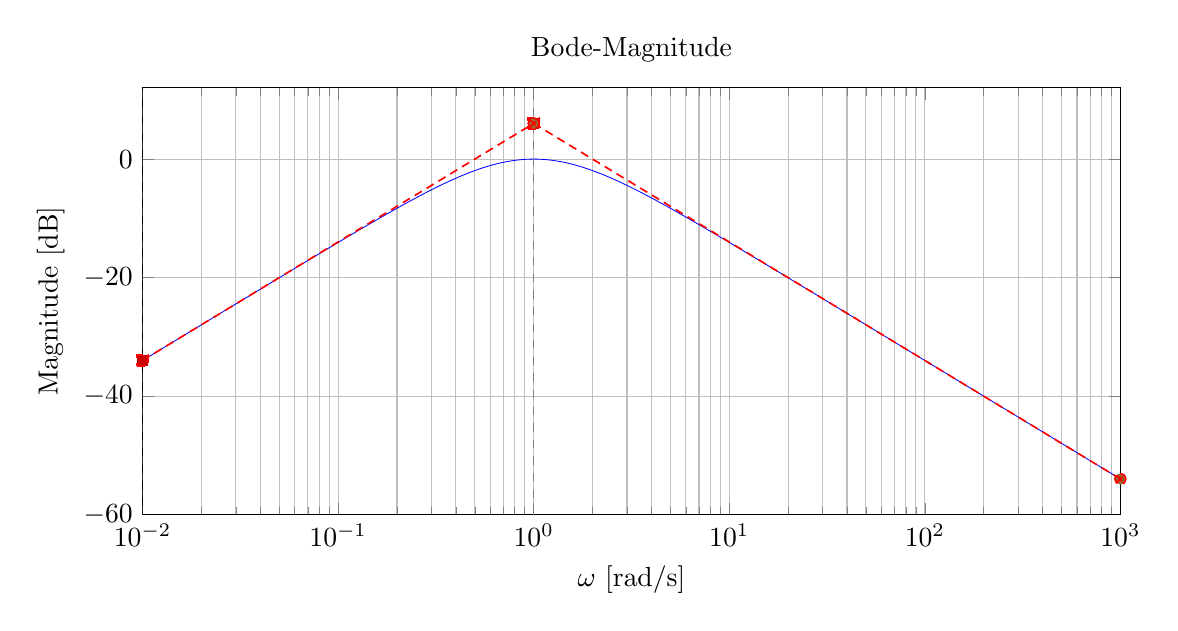
\begin{tikzpicture}
\begin{semilogxaxis}[
  width=14cm,height=7cm,
  xmin=1e-2,xmax=1e3,
  ytick distance=20,
  xlabel={$\omega$ [rad/s]},
  ylabel={Magnitude [dB]},
  grid=both,
  title={Bode-Magnitude}
]
\addplot[
  domain=1e-2:1e3,
  samples=700,
  mark=none,
  line width=0.3pt,
  blue
] {20*ln(2)/ln(10) + 20*ln(x)/ln(10) - 40*ln(sqrt(1 + x^2))/ln(10)};
\addplot+[domain=1e-2:1,samples=2,dashed,dash pattern=on 3pt off 2pt,line width=0.6pt,red] {20*ln(2)/ln(10) + 20*ln(x)/ln(10)};
\addplot+[domain=1:1e3,samples=2,dashed,dash pattern=on 3pt off 2pt,line width=0.6pt,red] {20*ln(2)/ln(10) - 20*ln(x)/ln(10)};
\draw[gray,dashed] (rel axis cs:0,0) -- (rel axis cs:0,1);
\draw[gray,dashed] (axis cs:1,\pgfkeysvalueof{/pgfplots/ymin}) -- (axis cs:1,\pgfkeysvalueof{/pgfplots/ymax});
\node[gray,anchor=south east] at (axis cs:1,\pgfkeysvalueof{/pgfplots/ymax}) {\scriptsize Pol $\omega_p=1$ (doppelt)};
\node[gray,anchor=south east] at (axis cs:1e-2,\pgfkeysvalueof{/pgfplots/ymax}) {\scriptsize Nullstelle im Ursprung};
\end{semilogxaxis}
\end{tikzpicture}
\vspace{6mm}
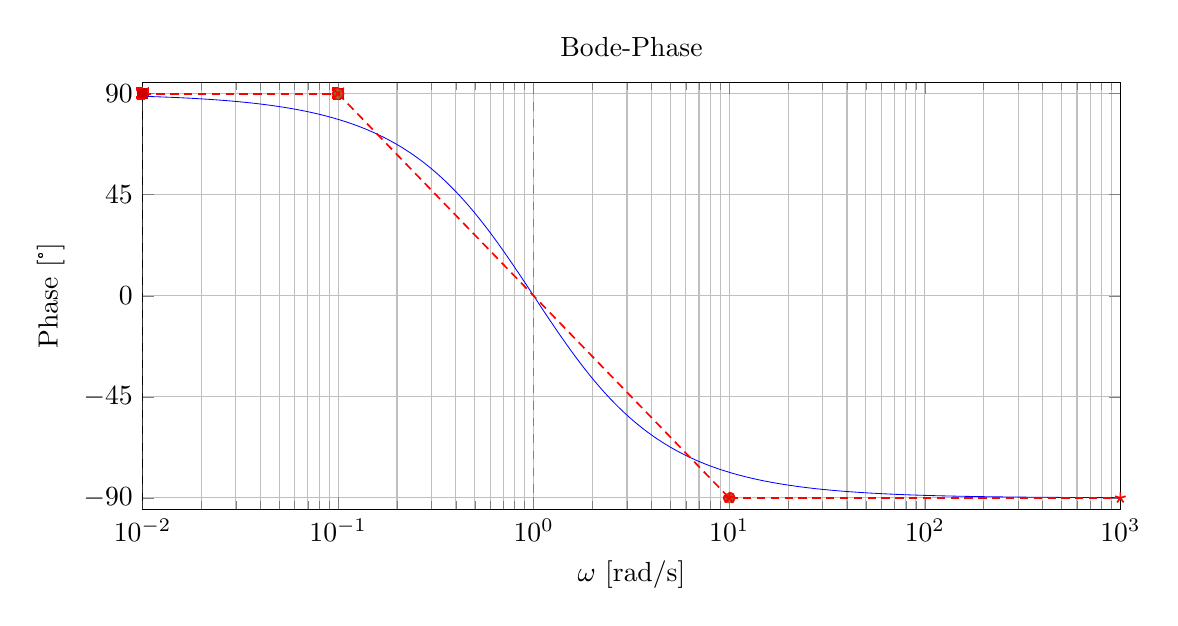
\begin{tikzpicture}
\begin{semilogxaxis}[
  width=14cm,height=7cm,
  xmin=1e-2,xmax=1e3,
  ymin=-95,ymax=95,
  ytick distance=45,
  xlabel={$\omega$ [rad/s]},
  ylabel={Phase [°]},
  grid=both,
  title={Bode-Phase}
]
\addplot[
  domain=1e-2:1e3,
  samples=700,
  mark=none,
  line width=0.3pt,
  blue
] {90 - 2*atan(x)};
\addplot+[domain=1e-2:1e-1,samples=2,dashed,dash pattern=on 3pt off 2pt,line width=0.6pt,red] {90};
\addplot+[domain=1e-1:1e1,samples=2,dashed,dash pattern=on 3pt off 2pt,line width=0.6pt,red] {45 - 90*ln(x)/ln(10) - 45};
\addplot+[domain=1e1:1e3,samples=2,dashed,dash pattern=on 3pt off 2pt,line width=0.6pt,red] {-90};
\draw[gray,dashed] (rel axis cs:0,0) -- (rel axis cs:0,1);
\draw[gray,dashed] (axis cs:1,\pgfkeysvalueof{/pgfplots/ymin}) -- (axis cs:1,\pgfkeysvalueof{/pgfplots/ymax});
\node[gray,anchor=south east] at (axis cs:1,\pgfkeysvalueof{/pgfplots/ymax}) {\scriptsize Pol $\omega_p=1$ (doppelt)};
\node[gray,anchor=south east] at (axis cs:1e-2,\pgfkeysvalueof{/pgfplots/ymax}) {\scriptsize Nullstelle im Ursprung};
\end{semilogxaxis}
\end{tikzpicture}
\end{center}
\newpage
\subsection{Erklärung (ausführlich)}
\begin{description}[leftmargin=1.2em,labelsep=.6em,font=\bfseries]

\item[1. Normalform herstellen.]
\[
H(s)=\frac{2s}{(s+1)^2}
=K_0\cdot s^{\,r}\cdot \frac{1}{(1+sT_p)^2}
\]
mit
\[
K_0=2,\quad r=1\ (\text{Nullstelle im Ursprung}),\quad T_p=1\ (\text{Doppelpol bei } \omega_p=1).
\]
Teilglieder:  \(\underline{F}_1(s)=\frac{1}{(1+s)^2}\) (reelles Polglied 2. Ordnung).

\item[2. Eckfrequenz bestimmen und sortieren.]
\[
\omega_p=\frac{1}{T_p}=1\,\mathrm{rad/s}.
\]
Nur diese Eckfrequenz; Sortierung trivial.

\item[3. Startpunkt des Amplitudengangs festlegen (Geradennäherung).]
Setze \(\omega_{\min}=\omega_p=1\). Skript-Regel:
\[
F_{\mathrm{dB}}(\omega_{\min})=20\log_{10}\!\big(|K_0\,\underline{F}_{ges}^*(0)|\cdot \omega_{\min}^{\,r}\big)
=20\log_{10}(2\cdot 1\cdot 1)=20\log_{10}2\approx +6\,\mathrm{dB}.
\]
Ankerpunkt der Geraden: \(+6\,\mathrm{dB}\) bei \(\omega=1\).

\item[4. Verlauf links vom Startpunkt zeichnen.]
Für \(\omega<1\) gilt Anfangssteigung \(r\cdot 20\,\mathrm{dB/dec}=+20\,\mathrm{dB/dec}\) (Nullstelle im Ursprung). Zeichne links vom Ankerpunkt eine Gerade mit \(+20\,\mathrm{dB/dec}\).

\item[5. Steigungswechsel an der Eckfrequenz eintragen.]
Doppelpol bei \(\omega=1\) bewirkt \(-40\,\mathrm{dB/dec}\) ab \(\omega=1\). Netto-Steigung:
\[
\begin{cases}
+20\,\mathrm{dB/dec},& \omega<1,\\
-20\,\mathrm{dB/dec},& \omega>1
\end{cases}
\]
(d.\,h.\ zwischen \(1\) und \(\infty\) fällt die Gerade mit \(-20\,\mathrm{dB/dec}\)).

\item[6. Eckabrundung korrekt berücksichtigen.]
Am Knick eines Doppelpols: \(-6\,\mathrm{dB}\) unter der Geradennäherung.
\[
|H(\j1)|_{\mathrm{dB}}\approx \underbrace{20\log_{10}2}_{\approx+6}\;-\;6=0\,\mathrm{dB}.
\]

\item[7. Phasenstartwert festlegen.]
Regel mit Vorzeichen und Ursprungsnull:
\[
K_0\,\underline{F}_{ges}^*(0)>0,\quad r=1
\;\Rightarrow\;
\varphi(0)=r\cdot 90^\circ=1\cdot 90^\circ=+90^\circ.
\]

\item[8. Phasenänderung durch Nullstelle und Doppelpol eintragen.]
Die Nullstelle im Ursprung liefert einen \emph{konstanten} Offset von \(+90^\circ\). Der Doppelpol bewirkt \(-180^\circ\) über die zwei Dekaden \([0.1,10]\) (je Pol \(-90^\circ\)). 
\textbf{Überlappung/Addierung:} In der Übergangszone \([0.1,10]\) wirken beide Polbeiträge gleichzeitig und addieren ihre Steigungen (insgesamt \(-90^\circ/\text{dec}\)). Der Offset \(+90^\circ\) der Ursprungsnull bleibt währenddessen konstant. Damit fällt die Phase von \(+90^\circ\) (für \(\omega\ll0.1\)) über \(0^\circ\) (bei \(\omega\approx1\)) weiter auf \(-90^\circ\) (für \(\omega\gg10\)). Näherung:
\[
\varphi(\omega)\approx
\begin{cases}
+90^\circ,& \omega\le 0.1,\\[2pt]
\;\;0^\circ-90^\circ\log_{10}\omega,& 0.1<\omega<10,\\[2pt]
-90^\circ,& \omega\ge 10.
\end{cases}
\]

\item[9. Grenzwerte und Konsistenz prüfen.]
DC: \(|H(0)|=0\Rightarrow -\infty\,\mathrm{dB}\), \(\varphi(0)=+90^\circ\).
HF: \(|H(\j\omega)|\sim 2/\omega\Rightarrow 20\log_{10}2-20\log_{10}\omega\,\mathrm{dB}\), \(\varphi(\infty)=(r-2)\cdot90^\circ=(1-2)\cdot90^\circ=-90^\circ\) (Pol-/Nullzählung konsistent).

\end{description}

\subsubsection*{Stückweise Näherungen (für die Skizze)}
\[
|H(j\omega)|_{\mathrm{dB}}\approx
\begin{cases}
20\log_{10}2+20\log_{10}\omega,& \omega\ll 1,\\[2pt]
\bigl(20\log_{10}2\bigr)-6=0,& \omega=1,\\[2pt]
20\log_{10}2-20\log_{10}\omega,& \omega\gg 1,
\end{cases}
\]\[
\varphi(\omega)\approx
\begin{cases}
+90^\circ,& \omega\le 0.1,\\[2pt]
0^\circ-90^\circ\log_{10}\omega,& 0.1<\omega<10,\\[2pt]
-90^\circ,& \omega\ge 10.
\end{cases}
\]
\newpage